%  A simple AAU report template.
%  2015-05-08 v. 1.2.0
%  Copyright 2010-2015 by Jesper Kjær Nielsen <jkn@es.aau.dk>
%
%  This is free software: you can redistribute it and/or modify
%  it under the terms of the GNU General Public License as published by
%  the Free Software Foundation, either version 3 of the License, or
%  (at your option) any later version.
%
%  This is distributed in the hope that it will be useful,
%  but WITHOUT ANY WARRANTY; without even the implied warranty of
%  MERCHANTABILITY or FITNESS FOR A PARTICULAR PURPOSE.  See the
%  GNU General Public License for more details.
%
%  You can find the GNU General Public License at <http://www.gnu.org/licenses/>.
%
% !TEX root = ../master.tex
\pdfbookmark[0]{Front page}{label:frontpage}%
\begin{titlepage}
  \addtolength{\hoffset}{0.5\evensidemargin-0.5\oddsidemargin} %set equal margins on the frontpage - remove this line if you want default margins
  \noindent%
  \begin{tabular}{@{}p{\textwidth}@{}}
    \toprule[2pt]
    \midrule
    \vspace{0.2cm}
    \begin{center}
    \Huge{\textbf{
      C Timed Information Flow% insert your title here
    }}
    \end{center}
    % \begin{center}
    %   \Large{
    %     - A Practical Approach -% insert your subtitle here
    %   }
    % \end{center}
    \vspace{0.2cm}\\
    \midrule
    \toprule[2pt]
  \end{tabular}
  \vspace{4 cm}
  \begin{center}
    {\large
      Master's Thesis%Insert document type (e.g., Project Report)
    }\\
    \vspace{0.2cm}
    {\Large %Insert your group name or real names here
      Mikael Elkiær Christensen\\
      Mikkel Sandø Larsen
    }
    \\[2.5cm]
    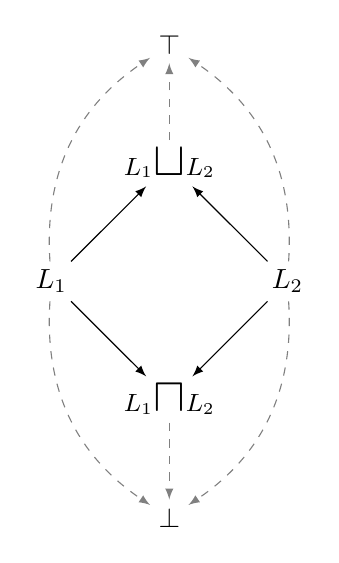
\begin{tikzpicture}[inner sep=1mm, >=latex, scale=1.5]
      \node (l1) at (-1,0) {$L_1$};
      \node (l2) at (1,0) {$L_2$};

      \node (meet) at (0,-1) {\small $L_1$ {\LARGE $\! \sqcap \!$} $L_2$};
      \node (bot) at (0,-2) {$\bot$};

      \node (join) at (0,1) {\small $L_1$ {\LARGE $\! \sqcup \!$} $L_2$};
      \node (top) at (0,2) {$\top$};

      \draw[->] (l1) edge (join);
      \draw[->] (l2) edge (join);
      \draw[->] (l1) edge (meet);
      \draw[->] (l2) edge (meet);

      \draw[->, dashed, gray] (l1) edge [bend left] (top);
      \draw[->, dashed, gray] (join) edge (top);
      \draw[->, dashed, gray] (l2) edge [bend right] (top);

      \draw[->, dashed, gray] (l1) edge [bend right] (bot);
      \draw[->, dashed, gray] (meet) edge (bot);
      \draw[->, dashed, gray] (l2) edge [bend left] (bot);
    \end{tikzpicture}
  \end{center}
  \vfill
  \begin{center}
  Aalborg University\\
  Department of Computer Science
  \end{center}
\end{titlepage}
\clearpage
